\documentclass{article}
\usepackage[utf8]{inputenc}
\usepackage[american]{babel}
\usepackage{csquotes}
\usepackage{hyperref}
\usepackage[backend=biber,style=numeric,hyperref=true,natbib=true,autocite=plain,sorting=none]{biblatex}

% gantt chart
\usepackage{pgfgantt}
\usepackage{rotating}
\usepackage[graphicx]{realboxes}

\newganttchartelement*{mymilestone}{
mymilestone/.style={
shape=isosceles triangle,
inner sep=0pt,
draw=cyan,
top color=white,
bottom color=cyan!50
},
mymilestone incomplete/.style={
/pgfgantt/mymilestone,
draw=yellow,
bottom color=yellow!50
},
mymilestone label font=\slshape,
mymilestone left shift=0pt,
mymilestone right shift=0pt
}

\newgantttimeslotformat{stardate}{%
\def\decomposestardate##1.##2\relax{%
\def\stardateyear{##1}\def\stardateday{##2}%
}%
\decomposestardate#1\relax%
\pgfcalendardatetojulian{\stardateyear-01-01}{#2}%
\advance#2 by-1\relax%
\advance#2 by\stardateday\relax%
}

% fix margins
\usepackage[margin=1in]{geometry}
\usepackage{fixltx2e}

% this package and the below text is to force images to be added to the given section and subsection. See https://tex.stackexchange.com/questions/279/how-do-i-ensure-that-figures-appear-in-the-section-theyre-associated-with/235312#235312 for more information
\usepackage{placeins}
\let\Oldsection\section
\renewcommand{\section}{\FloatBarrier\Oldsection}

\let\Oldsubsection\subsection
\renewcommand{\subsection}{\FloatBarrier\Oldsubsection}

\let\Oldsubsubsection\subsubsection
\renewcommand{\subsubsection}{\FloatBarrier\Oldsubsubsection}

\addbibresource{references.bib}

\title{%
  Design III Report: Bridge Structure \\
	\large Stevens Institute of Technology}

\date{October 2018}
\author{Joshua Schmidt, Andrew Chesterman, Jordan Balgahoom}

\usepackage{graphicx}

\begin{document}

\maketitle

\bigskip
\bigskip
\bigskip
\bigskip

\begin{figure}[!htb]
  \centering
  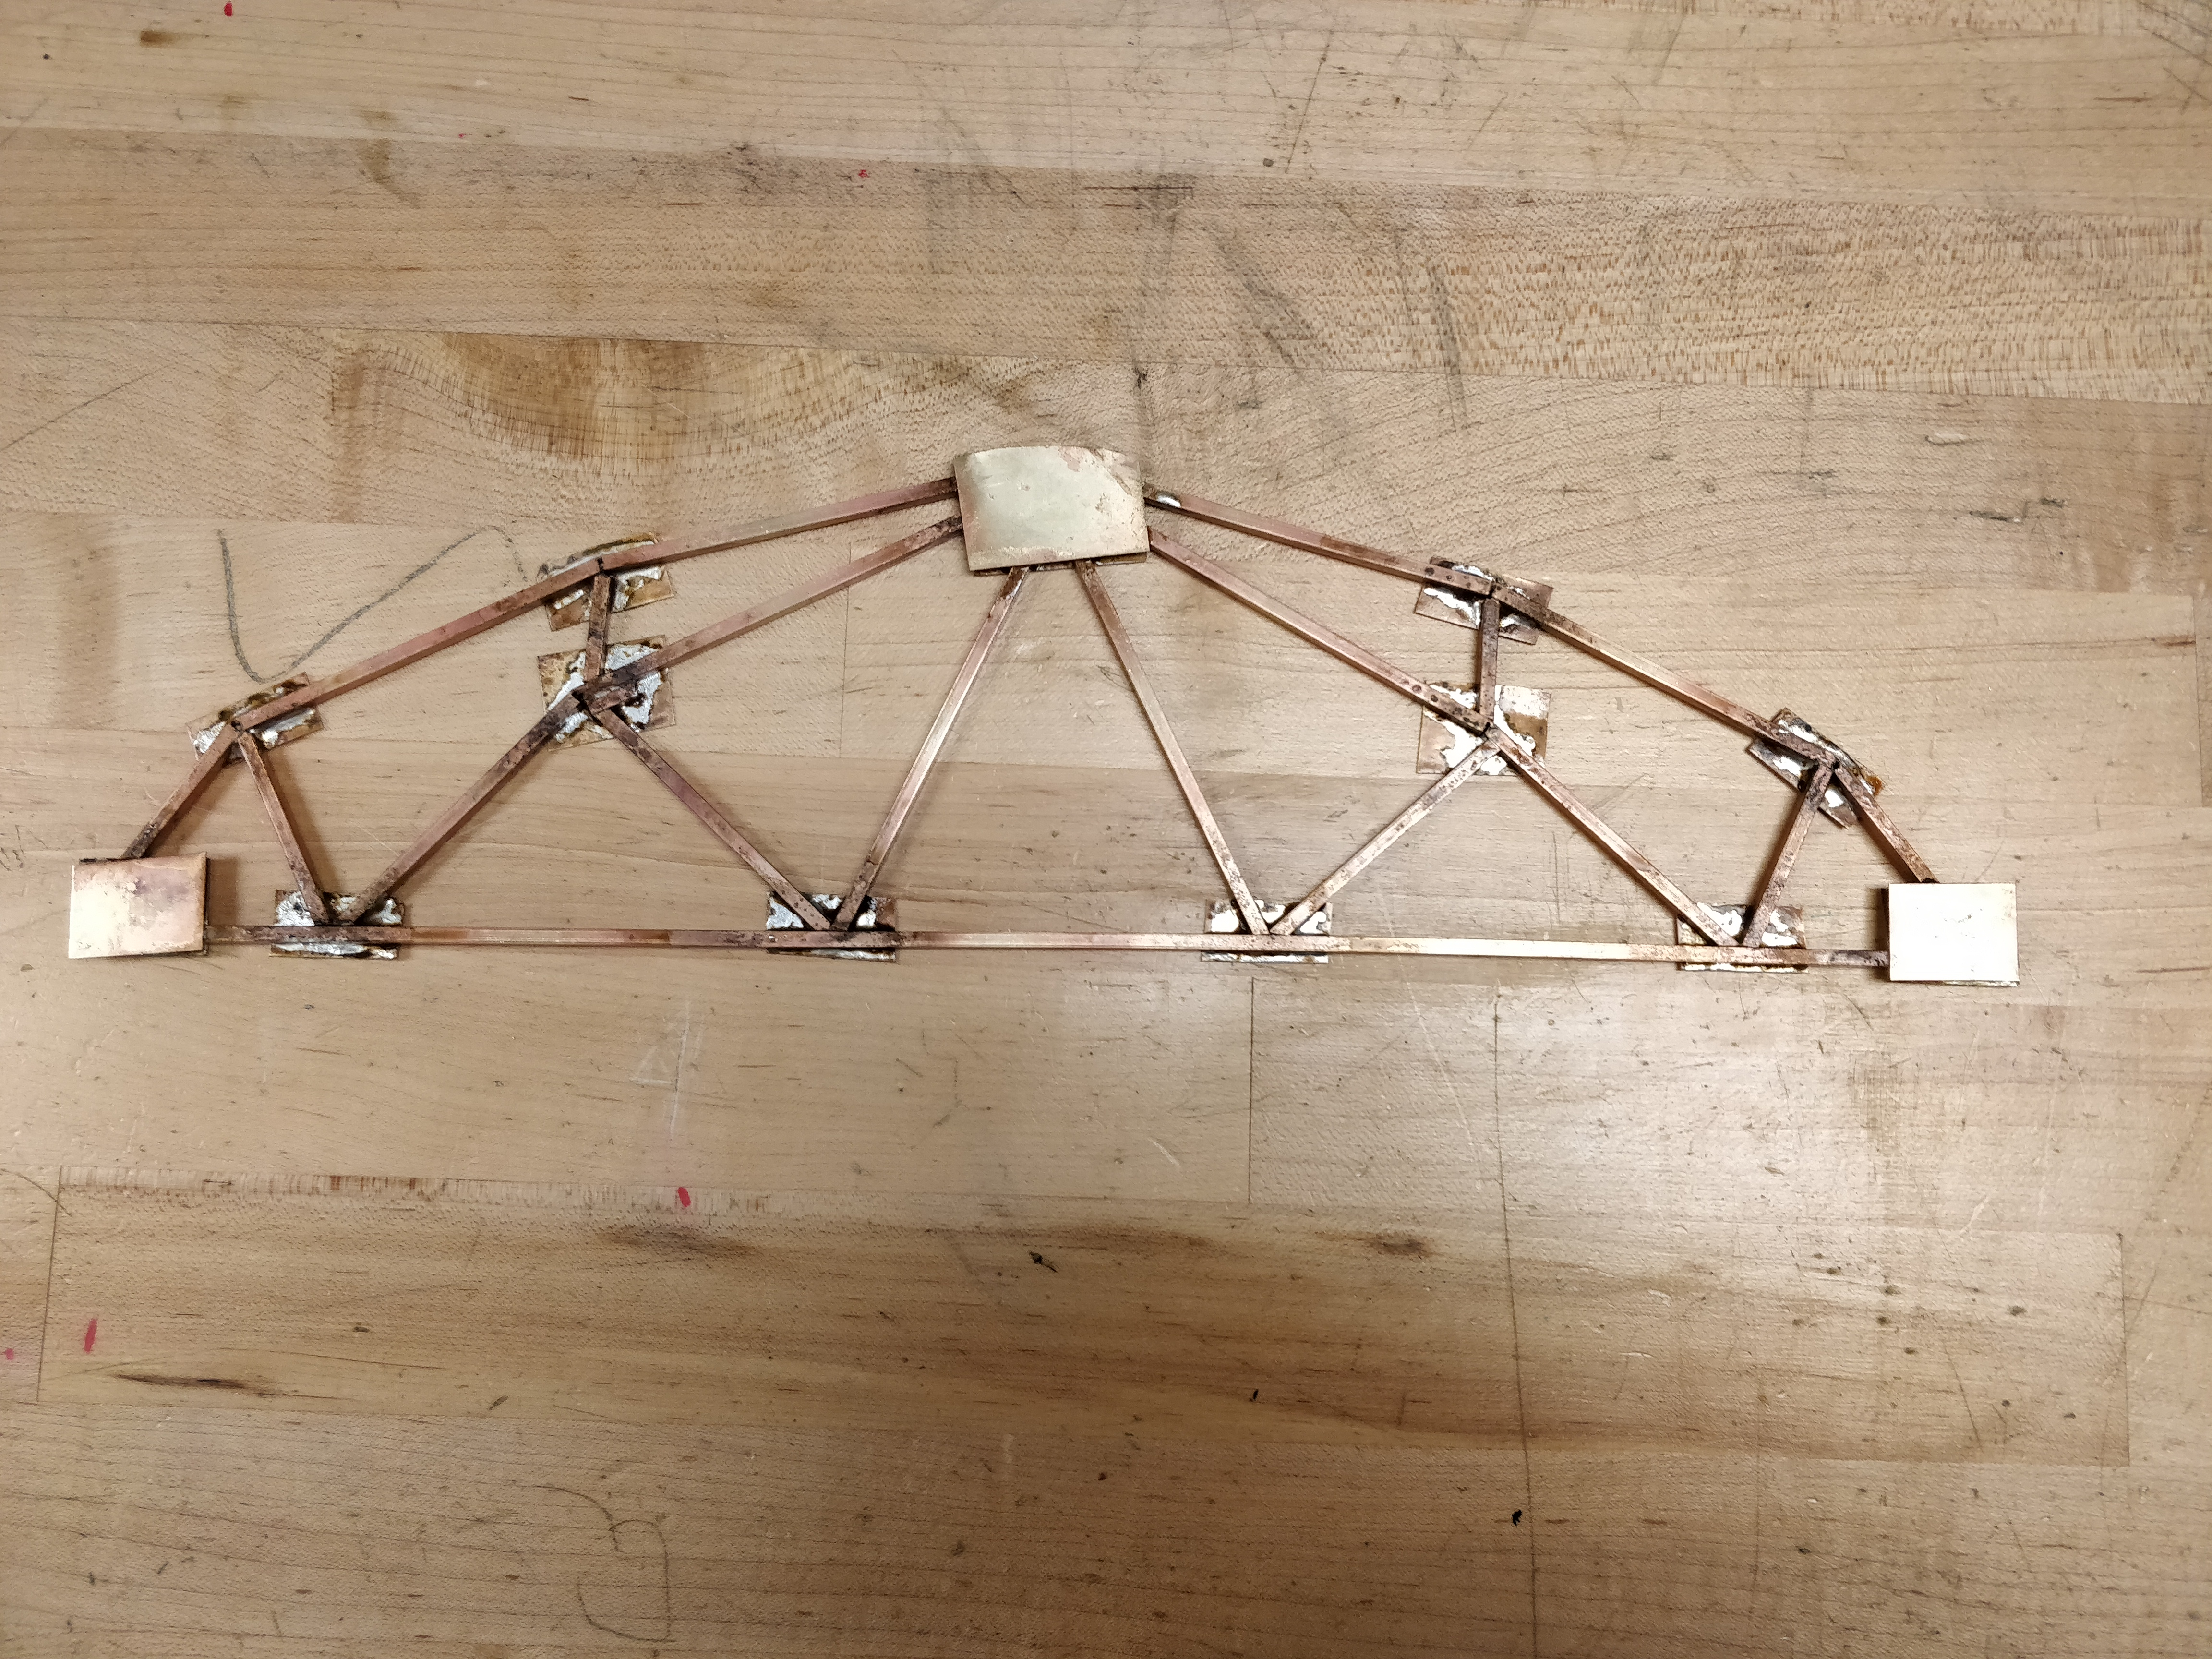
\includegraphics[width=0.75\textwidth]{assets/before-busting-side.jpg}
  \label{fig:logo}
\end{figure}

\newpage

\tableofcontents

\newpage

% References to all attachments in the main body of the report

\section{Abstract}

The goal of this project was to create a two-dimensional structure that can has the highest support-force to material-length ratio. The minimum load that the structure needed to support was 325 lbf, with a maximum copper tubing material length of 70 cm. The final load to length ratio was 6.8, with a maximum supported load of 475 lbf and a length of 66.2 inches. Therefore, this project was successful in meeting and surpassing the original specified requirements.

\newpage

\section{Introduction}

\subsection{Project objectives}

The main objective of this project was to design a planar truss that could support a given load over a given distance. Each team member had to design their own individual truss design before designing one final truss that would be used for testing. The final truss design was chosen because of its high load to failure, low amount of required material, and high strength to weight ratio. After all of these considerations, the truss was assembled by the team using the tools and materials provided to them.  

Project objectives (i.e. design, build, final truss selection: e.g highest load to failure; lowest material; best strength to weight; etc.)

\subsection{Project Specifications}

\subsubsection{Requirements}

The truss had to support a minimum of 325 lb, and a maximum of 500 lb. It had to be no more than 4" in height, and had to span a 15" gap. It could not exceed 2" below the horizontal span. In addition, the truss had to rest flat on two 1/2" wide supports in the truss buster. The joints at the supports, and the joint where the load would be applied, all had to be double gusseted. The joint that would bear the load also had to be at the top of the truss. The truss had to be no thicker than 0.175" at any given point, otherwise it would not fit in the truss buster. 

\subsubsection{Materials}
\begin{itemize}
\item Full Scale Paper Template
\item (2)x 36" Long, 1/8" Square Brass Tubing
\item (1)x 12" Long, 0.016" x 1" Brass Strip
\item Butane Torch
\item Flux Paste
\item Flux Brush
\item Refractory Bricks
\item Fume Extractor
\item Bandsaw/Hacksaw
\item Sander/Sandpaper
\item Lead-Free Solder
\item Heat Resistant Mat
\item Safety Goggles
\item Gloves
\item Hand Shear
\end{itemize}

\subsection{Approach}

The team stuck to the general schedule that was provided to the class. Design and construction took two class periods each. Testing was done on the last day of construction as well. 

Approach to project planning, scheduling, and completion.

\begin{figure}[!htb]
  \centering
  \includegraphics[width=0.75\textwidth]{assets/logo.png}
  \caption{scheduling chart}
  \label{fig:spacesuitdisplay}
\end{figure}

\newpage

\section{Discussion}

Introductory paragraph to Design Section content

\subsection{Design}

\subsubsection{Overview}

The team began designing their truss by experimenting in the Truss Analyzer application on the VLE. After some introduction to trusses in class, they played around with different designs to figure out what worked and what did not. They went through a few different  After much discussion and collaboration, they decided on their final design.
Overview of the design process

\subsubsection{Choice and Reasoning}

Each member of the team created their own trusses in the Truss Analyzer program on the VLE. The truss that was chosen out of the three individual truss designs was chosen due to its ability to hold more weight and use less material than the other two designs. While there was some concern due to the six member joint, the team chose this design anyway due to the effectiveness and efficiency of the design. This design also met the strength to length ratio for a full bonus two points on the design. The alternative designs held less weight than the chosen design and while they were simpler to build, they used more material than the chosen design, leaving less room for error. 

Truss design with alternatives considered in insight into your design decisions

\subsubsection{Design Analysis summary}



Design analysis summary as developed from Truss Analyzer with interpretation of data

\subsubsection{Fabrication}

One fabrication concern was the six member joint at the top of the truss. The more members that meet at a joint, the harder it is to solder. The team considered the difficulty of soldering this joint, and decided that, with enough practice, including the six member joint would greatly increase the strength of the truss.

Fabrication concerns and considerations in the design phase

\newpage

\section{Conclusion and Recommendations}

\subsection{Accomplishments}

The max load of the truss was 475 lb, which not only met, but exceeded the objective of the project. This max load was also far higher than the projected max load calculated by the truss analyzer. 66.2" of brass tubing was used, which was well under the maximum of 72". The truss also had a weight of 90g, which was 4th best in the class. In addition, the team was able to successfully solder the initially very daunting 6 member joint, which did not break at all during testing. The method of cutting at joints for many of the members was also a success because it allowed for easier construction and a stronger truss.

Describes the work in terms of accomplishments, both successful and unsuccessful

\subsection{Recommendations}

Given the opportunity to redo the project, the team would do a few things differently. First of all, measurements would be more accurate. Initially, when drawing the design of paper, the width of the brass tubes was not accounted for, so the truss construction went a little bit differently than expected. Another likely change would be more soldering practice. With more practice, the joints would have been slightly stronger, especially at the double gusset joints. Also, less solder would be used, which would decrease the weight and increase the strength to weight ratio of the truss.

Provides recommendations to improve the project in terms of basic knowledge, materials, equipment, or other guidance

Discuss what you would have done differently given the opportunity

\newpage

\section{Attachments}

\subsection{Work Chart}

Work break down structure and organization chart with roles and responsibilities

\begin{sidewaysfigure}
\begin{ganttchart}[vgrid, hgrid]{1}{12}
\gantttitle{September}{4} % by week or by day?
\gantttitle{October}{4} % October, November. Phase 1, 2, 3
\gantttitle{November}{4}\\
\gantttitlelist{1,...,12}{1}\\
%First Group
\ganttgroup{Group 1}{1}{10} \\
\ganttbar{Task 1}{2}{3} \\
\ganttbar{Task 2}{4}{10} \\
\ganttbar{Task 3}{9}{12}\\
%\ganttlink{elem0}{elem1}
\ganttlink{elem1}{elem2}
\ganttlink{elem2}{elem3}
%\ganttmilestone{Milestone 1}{11}
%Second Group
%\ganttgroup{Group 2}{14}{20} \\
%\ganttbar{Task 1}{15}{18} \\
%\ganttbar{Task 2}{18}{21} \\
%\ganttbar{Task 3}{22}{24}\\
%\ganttlink{elem4}{elem5}
%\ganttlink{elem5}{elem6}
%\ganttlink{elem6}{elem7}
%\ganttmilestone{Milestone 1}{11}
%Third Group
%\ganttgroup{Group 3}{25}{27} \\
%\ganttbar{Task 1}{26}{28} \\
%\ganttbar{Task 2}{28}{32} \\
%\ganttbar{Task 3}{32}{35}
%\ganttlink{elem8}{elem9}
%\ganttlink{elem9}{elem10}
%\ganttlink{elem10}{elem11}
%\ganttmilestone{Milestone 1}{11}
\end{ganttchart}
\end{sidewaysfigure}

\newpage

\subsection{Truss Analysis}

Truss Analysis jpg and csv printouts for final truss design

\newpage

\subsection{Alternatives Truss Analysis}

Truss Analysis jpg and csv printouts for at least two alternate designs considered

\newpage

\subsection{Data}

Brass compression data, charts, and formulas

\newpage

\printbibliography

\end{document}
